\documentclass[twoside, 10pt]{article}

\usepackage{geometry}
\geometry{outer=3em, inner=2.2cm, top=6em, bottom=4em, headheight=\paperheight}
\usepackage[export]{adjustbox}
\usepackage{array}
\usepackage{amsmath}
\usepackage{amsfonts}
\usepackage{fancyhdr}
\pagestyle{fancy}
\fancyhf{}
\lhead{Algebra II - BASE}
\chead{Business Applications/Domains and Ranges}
\rhead{Action Opportunity A, Page \thepage}
\usepackage{lastpage}
\usepackage{xcolor}
\usepackage{enumitem}
\usepackage{pifont}
\usepackage{graphicx}
\graphicspath{{../img}}
\usepackage{pgfplots}
\pgfplotsset{compat=1.18}
\usepackage{tabularx}
\usepackage{tikz}
\usetikzlibrary{patterns}

\newcommand{\R}{\mathbb R}
\newcommand{\e}{{\rm e}}
\newcommand{\pobr}[1]{\left\langle#1\right\rangle}
\newcommand{\norm}[1]{\lVert #1 \rVert}
\newcommand{\abs}[1]{\lvert #1 \rvert}

\DeclareMathOperator{\xd}{d\!}
\DeclareMathOperator{\proj}{proj}

\title{}
\date{}

\begin{document}
\noindent
{\large
First Name \rule{6em}{.1pt}\hspace{\stretch{1}}Last Name \rule{6em}{.1pt}\hspace{\stretch{1}} Date \rule{1.5em}{.1pt} -- \rule{1.5em}{.1pt} -- \rule{1.5em}{.1pt}\hspace{\stretch{1}} Period \rule{2em}{.1pt}\hspace{\stretch{1}} Score \rule{2em}{.1pt}
}
\vspace{1em}

\begingroup
\renewcommand{\arraystretch}{1.5}
\begin{center}
\tiny
{
\begin{tabularx}{\textwidth}{|X|X|X|X|X|X|}
\hline
\bf MODEL & \centerline{Integrating} & \centerline{Applying} & \centerline{Practicing} & \centerline{Acquiring} & \centerline{Awaiting Evidence} \\
\hline
I can use math to model and solve real-world problems.&
Correctly identifies
important
quantities and
illustrates their
relationships using
diagrams, tables,
graphs, or
formulas.
Appropriate work is
shown with no
errors. The answer
includes units and
rounding as
appropriate to the
problem.
Explains how the
answer makes
sense in the
context of the
problem.
&Correctly identifies
important
quantities and
illustrates their
relationships using
diagrams, tables,
graphs, or
formulas.
Appropriate work is
shown with no
errors. The answer
includes units and
rounding as
appropriate to the
problem.
&Correctly identifies
important
quantities and
illustrates their
relationships using
diagrams, tables,
graphs, or
formulas.
Appropriate work is
shown with 1
COMPUTATIONAL
or ROUNDING
error.
&Correctly identifies
important
quantities and
attempts to
illustrate their
relationships using
diagrams, tables,
graphs, or formulas
Appropriate work is
shown with 1
CONCEPTUAL
error.
&Correctly identifies
important
quantities and
attempts to
illustrate their
relationships using
diagrams, tables,
graphs, or formulas
Appropriate work is
shown with more
than 1 conceptual
error.\\
\hline
\bf Criteria&\multicolumn{5}{l|}{\parbox[c][4em]{.8\textwidth}{}}\\
\hline
\end{tabularx}
}
\end{center}
\endgroup
\vspace{1em}

{\noindent\bf Problems.}

\begin{enumerate}[leftmargin=*]
\item
A manufacturer of sweatshirts finds that profits and costs fluctuate depending on the number
of products created. Creating more products doesn't always increase profits because it requires
additional costs, such as building a larger facility or hiring more workers. The manufacturer
determines the profit, $p(x)$, in thousands of dollars, as a function of the number of sweatshirts
sold, $x$, in thousands. This function, $p$, is given below.
\[
p(x) = -x^3+9.5x^2-4x-38
\]

Graph $y=p(x)$ over the interval $0\leq x \leq 9$ on the set of axes below.
\begin{center}
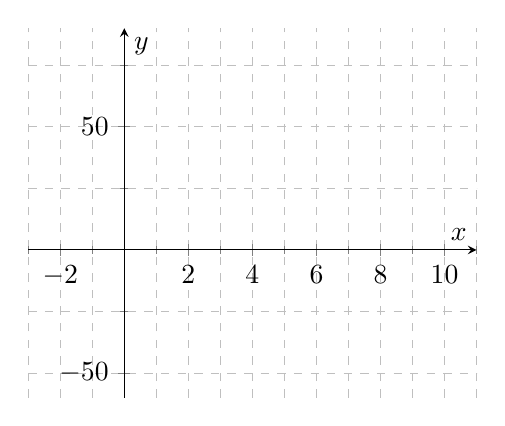
\begin{tikzpicture}
\begin{axis}[
axis lines=middle,
xmin=-3, xmax = 11,
xlabel={$x$}, ylabel={$y$},
ymin=-60, ymax=90,
domain=0:9,
grid=both,
minor tick num=1,
xtick distance = 2,
width=0.6\textwidth,
grid style={dashed}
]
\end{axis}
\end{tikzpicture}
\end{center}
Over the given interval, state the coordinates of the maximum of $p$ and round all values to
the nearest integer. {\bf Explain what this point represents in terms of the number of sweatshirts sold
and profit.}
\vspace{\stretch{1}}
\clearpage

\begingroup
\renewcommand{\arraystretch}{1.5}
\begin{center}
\tiny
{
\begin{tabularx}{\textwidth}{|X|X|X|X|X|X|}
\hline
\bf BE PRECISE & \centerline{Integrating} & \centerline{Applying} & \centerline{Practicing} & \centerline{Acquiring} & \centerline{Awaiting Evidence} \\
\hline
I can calculate accurately and efficiently, and be precise in all of my math.&
Selects and applies the correct procedure and solves all routine AND integrating problems.

AND

Expresses the answer to the correct level of precision needed for the problem (including the correct rounding, units, math symbols, labeling, graphing, vocab…)
&Selects and applies the correct procedure and solves all routine problems.


AND

Expresses the answer to the correct level of precision needed for the problem (including the correct rounding, units, math symbols, labeling, graphing, vocab…)
&Selects and applies the correct procedure and solves most routine problems.


AND

Expresses the answer to the correct level of precision needed for the problem (including the correct rounding, units, math symbols, labeling, graphing, vocab…)
&Selects and applies the correct procedure and solves some routine problems.


AND

Attempts to express the answer to the correct level of precision needed for the problem (including the correct rounding, units, math symbols, labeling, graphing, vocab…).
&Selects and attempts to apply the correct procedure for some routine problems.\\
\hline
\bf Criteria&\multicolumn{5}{l|}{\parbox[c][4em]{.8\textwidth}{}}\\
\hline
\end{tabularx}
}
\end{center}
\endgroup

\item Suppose $x$ is the width of a rectangle with length 10. The perimeter of the rectangle can be expressed as $P(x) = 2x + 20$. Find the domain and range of this perimeter function $P(x)$.
\vspace{1em}
\begin{itemize}
\item
Domain: \rule{0.5\textwidth}{.1pt}
\vspace{1em}
\item
Range: \rule{0.5\textwidth}{.1pt}
\end{itemize}
\item Find the domain and range from these points (written in set notation).
\begin{enumerate}
\item $\{(12,5), (3,67), (7,9), (0,3), (-1, 3)\}$
\vspace{1em}
\begin{itemize}
\item
Domain: $\{\rule{0.5\textwidth}{.1pt}\}$
\vspace{1em}
\item
Range: $\{\rule{0.5\textwidth}{.1pt}\}$ 
\end{itemize}
\item\ 

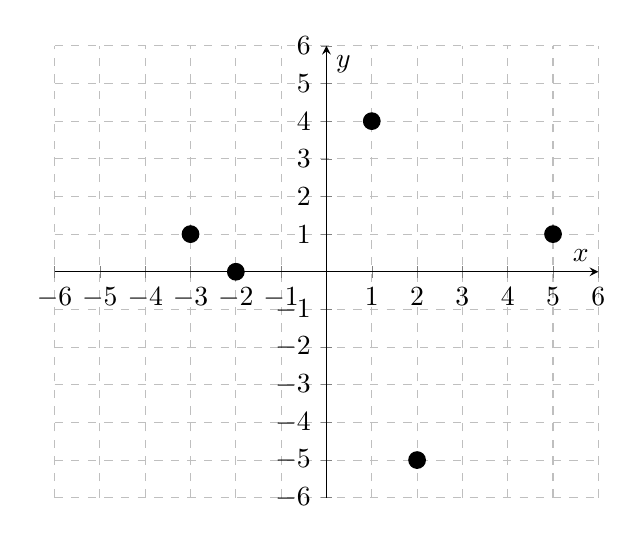
\begin{tikzpicture}
\begin{axis}[
axis lines=middle,
xmin=-6, xmax = 6,
xlabel={$x$}, ylabel={$y$},
ymin=-6, ymax=6,
grid=both,
xtick distance=1,
ytick distance=1,
width=0.7\textwidth,
grid style={dashed}
]
\draw[fill=black] (-2,0) circle (3pt);
\draw[fill=black] (-3,1) circle (3pt);
\draw[fill=black] (1,4) circle (3pt);
\draw[fill=black] (2,-5) circle(3pt);
\draw[fill=black] (5,1) circle(3pt);
\end{axis}
\end{tikzpicture}
\begin{itemize}
\item
Domain: $\{\rule{0.5\textwidth}{.1pt}\}$
\vspace{1em}
\item
Range: $\{\rule{0.5\textwidth}{.1pt}\}$ 
\end{itemize}
\end{enumerate}
\clearpage
\item Find the domain and range from a graph. Write them in interval notation or as an inequality.
\begin{enumerate}
\item\ 

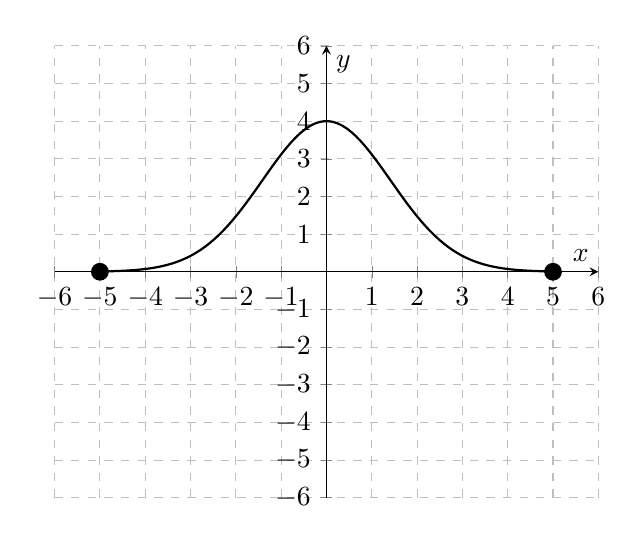
\begin{tikzpicture}
\begin{axis}[
axis lines=middle,
xmin=-6, xmax = 6,
xlabel={$x$}, ylabel={$y$},
ymin=-6, ymax=6,
grid=both,
xtick distance=1,
ytick distance=1,
width=0.7\textwidth,
grid style={dashed},
samples=100,
]
\addplot[thick]{4*e^(-(0.5*x)^2)};
\draw[fill=black] (5,0) circle(3pt);
\draw[fill=black] (-5,0) circle(3pt);
\end{axis}
\end{tikzpicture}
\begin{itemize}
\item
Domain: \rule{0.5\textwidth}{.1pt}
\vspace{1em}
\item
Range: \rule{0.5\textwidth}{.1pt}
\end{itemize}

\item\ 

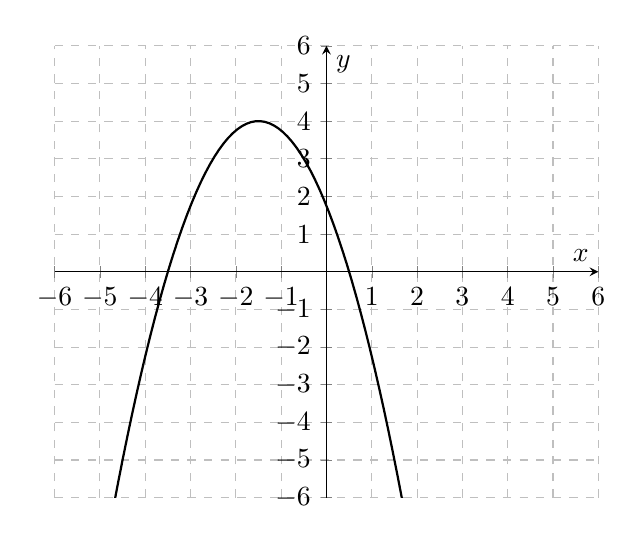
\begin{tikzpicture}
\begin{axis}[
axis lines=middle,
xmin=-6, xmax = 6,
xlabel={$x$}, ylabel={$y$},
ymin=-6, ymax=6,
grid=both,
xtick distance=1,
ytick distance=1,
width=0.7\textwidth,
grid style={dashed},
samples=100,
]
\addplot[thick]{-(x+4)*(x-1))-2.25};
\end{axis}
\end{tikzpicture}
\begin{itemize}
\item
Domain: \rule{0.5\textwidth}{.1pt}
\vspace{1em}
\item
Range: \rule{0.5\textwidth}{.1pt}
\end{itemize}
\end{enumerate}
\clearpage

\item Sketch functions that match the given domain and range.
\begin{enumerate}
\item
Domain: $-8\leq x\leq 3$, Range: $-1\leq y\leq 5$

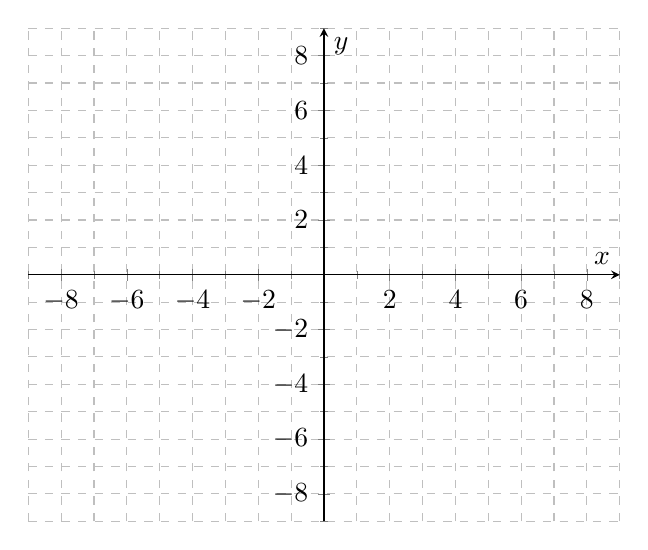
\begin{tikzpicture}
\begin{axis}[
axis lines=middle,
xmin=-9, xmax = 9,
xlabel={$x$}, ylabel={$y$},
ymin=-9, ymax=9,
grid=both,
xtick distance=2,
ytick distance=2,
minor tick num=1,
width=0.75\textwidth,
grid style={dashed},
samples=100,
]
\end{axis}
\end{tikzpicture}
\item
Domain: $-\infty <  x < \infty$, Range: $0 \leq y < \infty$

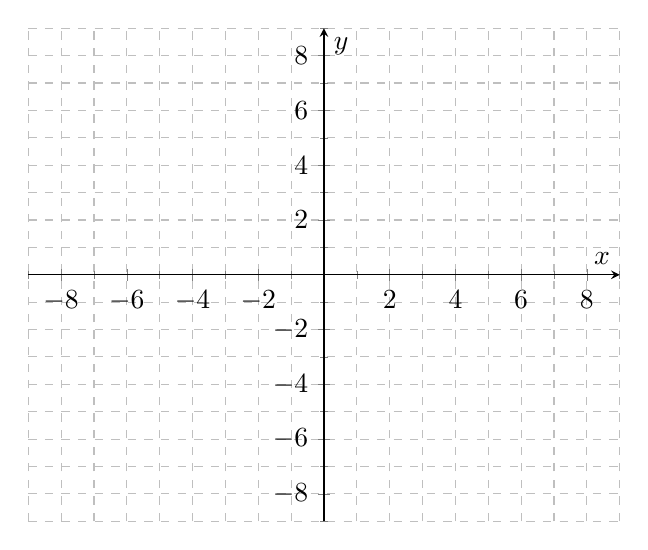
\begin{tikzpicture}
\begin{axis}[
axis lines=middle,
xmin=-9, xmax = 9,
xlabel={$x$}, ylabel={$y$},
ymin=-9, ymax=9,
grid=both,
xtick distance=2,
ytick distance=2,
minor tick num=1,
width=0.75\textwidth,
grid style={dashed},
samples=100,
]
\end{axis}
\end{tikzpicture}
\end{enumerate}
\end{enumerate}
\end{document}